\RequirePackage[l2tabu, orthodox]{nag}
\documentclass[french, english]{beamer}
%Permits to copy eg x ⪰ y ⇔ v(x) ≥ v(y) from PDF to unicode data, and to search. From pdfTeX users manual. See https://tex.stackexchange.com/posts/comments/1203887.
	\input glyphtounicode
	\pdfgentounicode=1
%Latin Modern has more glyphs than Computer Modern, such as diacritical characters. fntguide commands to load the font before fontenc, to prevent default loading of cmr.
	\usepackage{lmodern}
%Encode resulting accented characters correctly in resulting PDF, permits copy from PDF.
	\usepackage[T1]{fontenc}
%UTF8 seems to be the default in recent TeX installations, but not all, see https://tex.stackexchange.com/a/370280.
	\usepackage[utf8]{inputenc}
%Provides \newunicodechar for easy definition of supplementary UTF8 characters such as → or ≤ for use in source code.
	\usepackage{newunicodechar}
%Text Companion fonts, much used together with CM-like fonts. Provides \texteuro and commands for text mode characters such as \textminus, \textrightarrow, \textlbrackdbl.
	\usepackage{textcomp}
%St Mary’s Road symbol font, used for ⟦ = \llbracket.
	%\usepackage{stmaryrd}
%Solves bug in lmodern, https://tex.stackexchange.com/a/261188; probably useful only for unusually big font sizes; and probably better to use exscale instead. Note that the authors of exscale write against this trick.
	%\DeclareFontShape{OMX}{cmex}{m}{n}{
		%<-7.5> cmex7
		%<7.5-8.5> cmex8
		%<8.5-9.5> cmex9
		%<9.5-> cmex10
	%}{}
	%\SetSymbolFont{largesymbols}{normal}{OMX}{cmex}{m}{n}
%More symbols (such as \sum) available in bold version, see https://github.com/latex3/latex2e/issues/71.
	\DeclareFontShape{OMX}{cmex}{bx}{n}{%
	   <->sfixed*cmexb10%
	   }{}
	\SetSymbolFont{largesymbols}{bold}{OMX}{cmex}{bx}{n}
%For small caps also in italics, see https://tex.stackexchange.com/questions/32942/italic-shape-needed-in-small-caps-fonts, https://tex.stackexchange.com/questions/284338/italic-small-caps-not-working.
	\usepackage{slantsc}
	\AtBeginDocument{%
		%“Since nearly no font family will contain real italic small caps variants, the best approach is to substitute them by slanted variants.” -- slantsc doc
		%\DeclareFontShape{T1}{lmr}{m}{scit}{<->ssub*lmr/m/scsl}{}%
		%There’s no bold small caps in Latin Modern, we switch to Computer Modern for bold small caps, see https://tex.stackexchange.com/a/22241
		%\DeclareFontShape{T1}{lmr}{bx}{sc}{<->ssub*cmr/bx/sc}{}%
		%\DeclareFontShape{T1}{lmr}{bx}{scit}{<->ssub*cmr/bx/scsl}{}%
	}
%Warn about missing characters.
	\tracinglostchars=2
%Nicer tables: provides \toprule, \midrule, \bottomrule.
	%\usepackage{booktabs}
%For new column type X which stretches; can be used together with booktabs, see https://tex.stackexchange.com/a/97137. “tabularx modifies the widths of the columns, whereas tabular* modifies the widths of the inter-column spaces.” Loads array.
	%\usepackage{tabularx}
%math-mode version of "l" column type. Requires \usepackage{array}.
	%\usepackage{array}
	%\newcolumntype{L}{>{$}l<{$}}
%Provides \xpretocmd and loads etoolbox which provides \apptocmd, \patchcmd, \newtoggle… Also loads xparse, which provides \NewDocumentCommand and similar commands intended as replacement of \newcommand in LaTeX3 for defining commands (see https://tex.stackexchange.com/q/98152 and https://github.com/latex3/latex2e/issues/89).
	\usepackage{xpatch}
%ntheorem doc says: “empheq provides an enhanced vertical placement of the endmarks”; must be loaded before ntheorem. Loads the mathtools package, which loads and fixes some bugs in amsmath and provides \DeclarePairedDelimiter. amsmath is considered a basic, mandatory package nowadays (Grätzer, More Math Into LaTeX).
	\usepackage[ntheorem]{empheq}
%Package frenchb asks to load natbib before babel-french. Package hyperref asks to load natbib before hyperref.
	\usepackage{natbib}

\newtoggle{LCpres}
	\newtoggle{LCart}
	\newtoggle{LCposter}
	\makeatletter
	\@ifclassloaded{beamer}{
		\toggletrue{LCpres}
		\togglefalse{LCart}
		\togglefalse{LCposter}
		\wlog{Presentation mode}
	}{
		\@ifclassloaded{tikzposter}{
			\toggletrue{LCposter}
			\togglefalse{LCpres}
			\togglefalse{LCart}
			\wlog{Poster mode}
		}{
			\toggletrue{LCart}
			\togglefalse{LCpres}
			\togglefalse{LCposter}
			\wlog{Article mode}
		}
	}
	\makeatother%

%Language options ([french, english]) should be on the document level (last is main); except with tikzposter: put [french, english] options next to \usepackage{babel} to avoid warning. beamer uses the \translate command for the appendix: omitting babel results in a warning, see https://github.com/josephwright/beamer/issues/449. Babel also seems required for \refname.
	\iftoggle{LCpres}{
		\usepackage{babel}
	}{
	}
	%\frenchbsetup{AutoSpacePunctuation=false}
%listings (1.7) does not allow multi-byte encodings. listingsutf8 works around this only for characters that can be represented in a known one-byte encoding and only for \lstinputlisting. Other workarounds: use literate mechanism; or escape to LaTeX (but breaks alignment).
	%\usepackage{listings}
	%\lstset{tabsize=2, basicstyle=\ttfamily, escapechar=§, literate={é}{{\'e}}1}
%I favor acro over acronym because the former is more recently updated (2018 VS 2015 at time of writing); has a longer user manual (about 40 pages VS 6 pages if not counting the example and implementation parts); has a command for capitalization; and acronym suffers a nasty bug when ac used in section, see https://tex.stackexchange.com/q/103483 (though this might be the fault of the silence package and might be solved in more recent versions, I do not know) and from a bug when used with cleveref, see https://tex.stackexchange.com/q/71364. However, loading it makes compilation time (one pass on this template) go from 0.6 to 1.4 seconds, see https://bitbucket.org/cgnieder/acro/issues/115.
	%\usepackage[single]{acro}
	%\DeclareAcronym{AMCD}{short=AMCD, long={Aide Multicritère à la Décision}}
\DeclareAcronym{AHP}{short=AHP, long={Analytic Hierarchy Process}}
\DeclareAcronym{AR}{short=AR, long={Argumentative Recommender}}
\DeclareAcronym{DA}{short=DA, long={Decision Analysis}}
\DeclareAcronym{DJ}{short=DJ, long={Deliberated Judgment}}
\DeclareAcronym{DM}{short=DM, long={Decision Maker}}
\DeclareAcronym{DP}{short=DP, long={Deliberated Preference}}
\DeclareAcronym{ECC}{short=ECC, long={Egalitarian Compromise Compatible}}
\DeclareAcronym{MAVT}{short=MAVT, long={Multiple Attribute Value Theory}}
\DeclareAcronym{MCDA}{short=MCDA, long={Multicriteria Decision Aid}}
\DeclareAcronym{MIP}{short=MIP, long={Mixed Integer Program}}
\DeclareAcronym{PCC}{short=PCC, long={Paretian Compromise Compatible}}
\DeclareAcronym{SCR}{short=SCR, long={Social Choice Rule}}
\DeclareAcronym{SEU}{short=SEU, long={Subjective Expected Utility}}


\iftoggle{LCpres}{
	%I favor fmtcount over nth because it is loaded by datetime anyway; and fmtcount warns about possible conflicts when loaded after nth.
	\usepackage{fmtcount}
	%For nice input of date of presentation. Must be loaded after the babel package. Has possible problems with srcletter: https://golatex.de/verwendung-von-babel-und-datetime-in-scrlttr2-schlaegt-fehlt-t14779.html.
	\usepackage[nodayofweek]{datetime}
}{
}
%For presentations, Beamer implicitely uses the pdfusetitle option. ntheorem doc says to load hyperref “before the first use of \newtheorem”. autonum doc mandates option hypertexnames=false. I want to highlight links only if necessary for the reader to recognize it as a link, to reduce distraction. In presentations, this is already taken care of by beamer (https://tex.stackexchange.com/a/262014). If using colorlinks=true in a presentation, see https://tex.stackexchange.com/q/203056. Crashes the first compilation with tikzposter, just compile again and the problem disappears, see https://tex.stackexchange.com/q/254257.
\makeatletter
\iftoggle{LCpres}{
	\usepackage{hyperref}
}{
	\usepackage[hypertexnames=false, pdfusetitle, linkbordercolor={1 1 1}, citebordercolor={1 1 1}, urlbordercolor={1 1 1}]{hyperref}
	%https://tex.stackexchange.com/a/466235
	\pdfstringdefDisableCommands{%
		\let\thanks\@gobble
	}
}
\makeatother
%urlbordercolor is used both for \url and \doi, which I think shouldn’t be colored, and for \href, thus might want to color manually when required. Requires xcolor.
	\NewDocumentCommand{\hrefblue}{mm}{\textcolor{blue}{\href{#1}{#2}}}
%hyperref doc says: “Package bookmark replaces hyperref’s bookmark organization by a new algorithm (...) Therefore I recommend using this package”.
	\usepackage{bookmark}
%Need to invoke hyperref explicitly to link to line numbers: \hyperlink{lintarget:mylinelabel}{\ref*{lin:mylinelabel}}, with \ref* to disable automatic link. Also see https://tex.stackexchange.com/q/428656 for referencing lines from another document.
	%\usepackage{lineno}
	%\NewDocumentCommand{\llabel}{m}{\hypertarget{lintarget:#1}{}\linelabel{lin:#1}}
	%\setlength\linenumbersep{9mm}
%For complex authors blocks. Seems like authblk wants to be later than hyperref, but sooner than silence. See https://tex.stackexchange.com/q/475513 for the patch to hyperref pdfauthor.
	\ExplSyntaxOn
	\seq_new:N \g_oc_hrauthor_seq
	\NewDocumentCommand{\addhrauthor}{m}{
		\seq_gput_right:Nn \g_oc_hrauthor_seq { #1 }
	}
	%Should be \NewExpandableDocumentCommand, but this is not yet provided by my version of xparse
	\DeclareExpandableDocumentCommand{\hrauthor}{}{
		\seq_use:Nn \g_oc_hrauthor_seq {,~}
	}
	\ExplSyntaxOff
	{
		\catcode`#=11\relax
		\gdef\fixauthor{\xpretocmd{\author}{\addhrauthor{#2}}{}{}}%
	}
	\iftoggle{LCart}{
		\usepackage{authblk}
		\renewcommand\Affilfont{\small}
		\fixauthor
		\AtBeginDocument{
		    \hypersetup{pdfauthor={\hrauthor}}
		}
	}{
	}
%I do not use floatrow, because it requires an ugly hack for proper functioning with KOMA script (see scrhack doc). Instead, the following command centers all floats (using \centering, as the center environment adds space, http://texblog.net/latex-archive/layout/center-centering/), and I manually place my table captions above and figure captions below their contents (https://tex.stackexchange.com/a/3253).
	\makeatletter
	\g@addto@macro\@floatboxreset\centering
	\makeatother
%Permits to customize enumeration display and references
	%\nottoggle{LCpres}{
		%\usepackage{enumitem} %follow list environments by a string to customize enumeration, example: \begin{description}[itemindent=8em, labelwidth=!] or \begin{enumerate}[label=({\roman*}), ref={\roman*}].
	%}{
	%}
%Provides \Centering, \RaggedLeft, and \RaggedRight and environments Center, FlushLeft, and FlushRight, which allow hyphenation. With tikzposter, seems to cause 1=1 to be printed in the middle of the poster.
	%\usepackage{ragged2e}
%To typeset units by closely following the “official” rules.
	%\usepackage[strict]{siunitx}
%Turns the doi provided by some bibliography styles into URLs. However, uses old-style dx.doi url (see 3.8 DOI system Proxy Server technical details, “Users may resolve DOI names that are structured to use the DOI system Proxy Server (https://doi.org (current, preferred) or earlier syntax http://dx.doi.org).”, https://www.doi.org/doi_handbook/3_Resolution.html). The patch solves this.
	\usepackage{doi}
	\makeatletter
	\patchcmd{\@doi}{http://dx.doi.org}{https://doi.org}{}{}
	\makeatother
%Makes sure upper case greek letters are italic as well.
	\usepackage{fixmath}
%Provides \mathbb; obsoletes latexsym (see http://tug.ctan.org/macros/latex/base/latexsym.dtx). Relatedly, \usepackage{eucal} to change the mathcal font and \usepackage[mathscr]{eucal} (apparently equivalent to \usepackage[mathscr]{euscript}) to supplement \mathcal with \mathscr. This last option is not very useful as both fonts are similar, and the intent of the authors of eucal was to provide a replacement to mathcal (see doc euscript). Also provides \mathfrak for supplementary letters.
	\usepackage{amsfonts}
%Provides a beautiful (IMHO) \mathscr and really different than \mathcal, for supplementary uppercase letters. But there is no bold version. Alternative: mathrsfs (more slanted), but when used with tikzposter, it warns about size substitution, see https://tex.stackexchange.com/q/495167.
	\usepackage[scr]{rsfso}
%Multiple means to produce bold math: \mathbf, \boldmath (defined to be \mathversion{bold}, see fntguide), \pmb, \boldsymbol (all legacy, from LaTeX base and AMS), \bm (the most recommended one), \mathbold from package fixmath (I don’t see its advantage over \boldsymbol).
%“The \boldsymbol command is obtained preferably by using the bm package, which provides a newer, more powerful version than the one provided by the amsmath package. Generally speaking, it is ill-advised to apply \boldsymbol to more than one symbol at a time.” — AMS Short math guide. “If no bold font appears to be available for a particular symbol, \bm will use ‘poor man’s bold’” — bm. It is “best to load the package after any packages that define new symbol fonts” – bm. bm defines \boldsymbol as synonym to \bm. \boldmath accesses the correct font if it exists; it is used by \bm when appropriate. See https://tex.stackexchange.com/a/10643 and https://github.com/latex3/latex2e/issues/71 for some difficulties with \bm.
	\usepackage{bm}
	\nottoggle{LCpres}{
	%https://ctan.org/pkg/amsmath recommends ntheorem, which supersedes amsthm, which corrects the spacing of proclamations and allows for theoremstyle. Option standard loads amssymb and latexsym. Must be loaded after amsmath (from ntheorem doc). From cleveref doc, “ntheorem is fully supported and even recommended”; says to load cleveref after ntheorem. When used with tikzposter, warns about size substitution for the lasy (latexsym) font when using \url, because ntheorem loads latexsym; relatedly (but not directly related to ntheorem), size substitution warning with the cmex font happens when loading amsmath and using \url. According to https://tex.stackexchange.com/q/535950, ntheorem “seems essentially unmaintaned and has severe problems”, but I use it anyway because it is very handy. Yields “! LaTeX Error: Something's wrong--perhaps a missing \item.” if some theorem follows thebibliography.
		\usepackage[thmmarks, amsmath, standard, hyperref]{ntheorem}
		%empheq doc says to do this after loading ntheorem
		\usetagform{default}
	%Provides \cref. Unfortunately, cref fails when the language is French and referring to a label whose name contains a colon (https://tex.stackexchange.com/q/83798). Use \cref{sec\string:intro} to work around this. cleveref should go “laster” than hyperref.
		\usepackage{cleveref}
	}{
	}
	\nottoggle{LCposter}{
	%Equations get numbers iff they are referenced. Loading order should be “amsmath → hyperref → cleveref → autonum”, according to autonum doc. Use this in preference to the showonlyrefs option from mathtools, see https://tex.stackexchange.com/q/459918 and autonum doc. See https://tex.stackexchange.com/a/285953 for the etex line. Incompatible with my version of tikzposter (produces “! Improper \prevdepth”).
		\expandafter\def\csname ver@etex.sty\endcsname{3000/12/31}\let\globcount\newcount
		\usepackage{autonum}
	}{
	}
%Also loaded by tikz.
	%\usepackage{xcolor}
\iftoggle{LCpres}{
	\usepackage{tikz}
	%\usetikzlibrary{babel, matrix, fit, plotmarks, calc, trees, shapes.geometric, positioning, plothandlers, arrows, shapes.multipart}
}{
}
%Vizualization, on top of TikZ
	%\usepackage{pgfplots}
	%\pgfplotsset{compat=1.14}
\usepackage{graphicx}
	\graphicspath{{graphics/}}

%Provides \printlength{length}, useful for debugging.
	%\usepackage{printlen}
	%\uselengthunit{mm}

\iftoggle{LCpres}{
	\usepackage{appendixnumberbeamer}
	%I have yet to see anyone actually use these navigation symbols; let’s disable them
	\setbeamertemplate{navigation symbols}{} 
	\usepackage{preamble/beamerthemeParisFrance}
	\setcounter{tocdepth}{10}
}{
}

%Do not use the displaymath environment: use equation. Do not use the eqnarray or eqnarray* environments: use align(*). This improves spacing. (See l2tabu or amsldoc.)


%Requires package xcolor.
\NewDocumentCommand{\commentOC}{m}{\textcolor{blue}{\small$\big[$OC: #1$\big]$}}
%Requires package babel and option [french]. According to babel doc, need two braces around \selectlanguage to make the changes really local.
\NewDocumentCommand{\commentOCf}{m}{\textcolor{blue}{{\small\selectlanguage{french}$\big[$OC : #1$\big]$}}}
\NewDocumentCommand{\commentYM}{m}{\textcolor{red}{\small$\big[$YM: #1$\big]$}}
\NewDocumentCommand{\commentYMf}{m}{\textcolor{red}{{\small\selectlanguage{french}$\big[$YM : #1$\big]$}}}

\bibliographystyle{abbrvnat}
\NewDocumentCommand{\possessivecite}{mO{}}{\citeauthor{#1}’s \citeyearpar[#2]{#1}}

%https://tex.stackexchange.com/a/467188, https://tex.stackexchange.com/a/36088 - uncomment if one of those symbols is used.
%\DeclareFontFamily{U} {MnSymbolD}{}
%\DeclareFontShape{U}{MnSymbolD}{m}{n}{
%  <-6> MnSymbolD5
%  <6-7> MnSymbolD6
%  <7-8> MnSymbolD7
%  <8-9> MnSymbolD8
%  <9-10> MnSymbolD9
%  <10-12> MnSymbolD10
%  <12-> MnSymbolD12}{}
%\DeclareFontShape{U}{MnSymbolD}{b}{n}{
%  <-6> MnSymbolD-Bold5
%  <6-7> MnSymbolD-Bold6
%  <7-8> MnSymbolD-Bold7
%  <8-9> MnSymbolD-Bold8
%  <9-10> MnSymbolD-Bold9
%  <10-12> MnSymbolD-Bold10
%  <12-> MnSymbolD-Bold12}{}
%\DeclareSymbolFont{MnSyD} {U} {MnSymbolD}{m}{n}
%\DeclareMathSymbol{\ntriplesim}{\mathrel}{MnSyD}{126}
%\DeclareMathSymbol{\nlessgtr}{\mathrel}{MnSyD}{192}
%\DeclareMathSymbol{\ngtrless}{\mathrel}{MnSyD}{193}
%\DeclareMathSymbol{\nlesseqgtr}{\mathrel}{MnSyD}{194}
%\DeclareMathSymbol{\ngtreqless}{\mathrel}{MnSyD}{195}
%\DeclareMathSymbol{\nlesseqgtrslant}{\mathrel}{MnSyD}{198}
%\DeclareMathSymbol{\ngtreqlessslant}{\mathrel}{MnSyD}{199}
%\DeclareMathSymbol{\npreccurlyeq}{\mathrel}{MnSyD}{228}
%\DeclareMathSymbol{\nsucccurlyeq}{\mathrel}{MnSyD}{229}
%\DeclareFontFamily{U} {MnSymbolA}{}
%\DeclareFontShape{U}{MnSymbolA}{m}{n}{
%  <-6> MnSymbolA5
%  <6-7> MnSymbolA6
%  <7-8> MnSymbolA7
%  <8-9> MnSymbolA8
%  <9-10> MnSymbolA9
%  <10-12> MnSymbolA10
%  <12-> MnSymbolA12}{}
%\DeclareFontShape{U}{MnSymbolA}{b}{n}{
%  <-6> MnSymbolA-Bold5
%  <6-7> MnSymbolA-Bold6
%  <7-8> MnSymbolA-Bold7
%  <8-9> MnSymbolA-Bold8
%  <9-10> MnSymbolA-Bold9
%  <10-12> MnSymbolA-Bold10
%  <12-> MnSymbolA-Bold12}{}
%\DeclareSymbolFont{MnSyA} {U} {MnSymbolA}{m}{n}
%%Rightwards wave arrow: ↝. Alternative: \rightsquigarrow from amssymb, but it’s uglier
%\DeclareMathSymbol{\rightlsquigarrow}{\mathrel}{MnSyA}{160}

%03B3 Greek Small Letter Gamma
\newunicodechar{γ}{\gamma}
%03B4 Greek Small Letter Delta
\newunicodechar{δ}{\delta}
%2115 Double-Struck Capital N
\newunicodechar{ℕ}{\mathbb{N}}
%211D Double-Struck Capital R
\newunicodechar{ℝ}{\mathbb{R}}
%21CF Rightwards Double Arrow with Stroke
\newunicodechar{⇏}{\nRightarrow}
%21D2 Rightwards Double Arrow
\newunicodechar{⇒}{\ensuremath{\Rightarrow}}
%21D4 Left Right Double Arrow
\newunicodechar{⇔}{\Leftrightarrow}
%21DD Rightwards Squiggle Arrow
\newunicodechar{⇝}{\rightsquigarrow}
%2205 Empty Set
\newunicodechar{∅}{\emptyset}
%2212 Minus Sign
\newunicodechar{−}{\ifmmode{-}\else\textminus\fi}
%2227 Logical And
\newunicodechar{∧}{\land}
%2228 Logical Or
\newunicodechar{∨}{\lor}
%2229 Intersection
\newunicodechar{∩}{\cap}
%222A Union
\newunicodechar{∪}{\cup}
%2260 Not Equal To (handy also as text in informal writing)
\newunicodechar{≠}{\ensuremath{\neq}}
%2264 Less-Than or Equal To
\newunicodechar{≤}{\leq}
%2265 Greater-Than or Equal To
\newunicodechar{≥}{\geq}
%2270 Neither Less-Than nor Equal To
\newunicodechar{≰}{\nleq}
%2271 Neither Greater-Than nor Equal To
\newunicodechar{≱}{\ngeq}
%2272 Less-Than or Equivalent To
\newunicodechar{≲}{\lesssim}
%2273 Greater-Than or Equivalent To
\newunicodechar{≳}{\gtrsim}
%2274 Neither Less-Than nor Equivalent To – also, from MnSymbol: \nprecsim, a more exact match to the Unicode symbol; and \npreccurlyeq, too small
\newunicodechar{≴}{\not\preccurlyeq}
%2275 Neither Greater-Than nor Equivalent To
\newunicodechar{≵}{\not\succcurlyeq}
%2279 Neither Greater-Than nor Less-Than – requires MnSymbol; also \nlessgtr from txfonts/pxfonts, \ngtreqless from MnSymbol (but much higher), \ngtrless from MnSymbol (a more exact match to the Unicode symbol); for incomparability (not matching this Unicode symbol), may also consider \ntriplesim from MnSymbol,\nparallelslant from fourier, \between from mathabx, or ⋈
\newunicodechar{≹}{\ngtreqlessslant}
%227A Precedes
\newunicodechar{≺}{\prec}
%227B Succeeds
\newunicodechar{≻}{\succ}
%227C Precedes or Equal To
\newunicodechar{≼}{\preccurlyeq}
%227D Succeeds or Equal To
\newunicodechar{≽}{\succcurlyeq}
%227E Precedes or Equivalent To
\newunicodechar{≾}{\precsim}
%227F Succeeds or Equivalent To
\newunicodechar{≿}{\succsim}
%2280 Does Not Precede
\newunicodechar{⊀}{\nprec}
%2281 Does Not Succeed
\newunicodechar{⊁}{\nsucc}
%22B2 Normal Subgroup Of – using \vartriangleleft from amsfonts, which goes well with \trianglelefteq, \ntriangleright, and so on, also from amsfonts; another possibility is \lhd from latexsym, which seems visually equivalent to \vartriangleleft from amsfonts; latexsym also has ⊴=\unlhd, but doesn’t have a symbol for ⊴. Other related symbols: \triangleleft from latesym package is too small; fdsymbol provides \triangleleft=\medtriangleleft and \vartriangleleft=\smalltriangleleft; MnSymbol provides \medtriangleleft and \vartriangleleft=\lessclosed=\lhd which are smaller than \vartriangleleft from amsfont; \vartriangleleft from mathabx (p. 67), looks different (wider); also \vartriangleleft from boisik (p. 69) looks still different; \vartriangleleft=\lhd from stix are smaller. Oddly enough, \triangleright appears as the LMMathItalic12-Regular font whereas \rhd appears as LASY10 and \vartriangleright appears as MSAM10.
\newunicodechar{⊲}{\vartriangleleft}
%22B3 Contains as Normal Subgroup (also: 25B7 White right-pointing triangle or 25B9 White right-pointing small triangle)
\newunicodechar{⊳}{\vartriangleright}
%22B4 Normal Subgroup of or Equal To
\newunicodechar{⊴}{\trianglelefteq}
%22B5 Contains as Normal Subgroup or Equal To
\newunicodechar{⊵}{\trianglerighteq}
%22C8 Bowtie
\newunicodechar{⋈}{\bowtie}
%22EA Not Normal Subgroup Of
\newunicodechar{⋪}{\ntriangleleft}
%22EB Does Not Contain As Normal Subgroup
\newunicodechar{⋫}{\ntriangleright}
%22EC Not Normal Subgroup of or Equal To
\newunicodechar{⋬}{\ntrianglelefteq}
%22ED Does Not Contain as Normal Subgroup or Equal
\newunicodechar{⋭}{\ntrianglerighteq}
%25A1 White Square
\newunicodechar{□}{\Box}
%27E6 Mathematical Left White Square Bracket – requires stmaryrd (alternative: \text{\textlbrackdbl}, but ugly if used in an italicized text such as a theorem)
\newunicodechar{⟦}{\llbracket}
%27E7 Mathematical Right White Square Bracket
\newunicodechar{⟧}{\rrbracket}
%27FC Long Rightwards Arrow from Bar
\newunicodechar{⟼}{\longmapsto}
%2AB0 Succeeds Above Single-Line Equals Sign
\newunicodechar{⪰}{\succeq}
%301A Left White Square Bracket
\newunicodechar{〚}{\textlbrackdbl}
%301B Right White Square Bracket
\newunicodechar{〛}{\textrbrackdbl}
%→ is defined by default as \textrightarrow, which is invalid in math mode. Same thing for the three other commands. Using \DeclareUnicodeCharacter instead of \newunicodechar because the latter warns about the previous definition.
%→ Rightwards Arrow
\DeclareUnicodeCharacter{2192}{\ifmmode\rightarrow\else\textrightarrow\fi}
%¬ Not Sign
\DeclareUnicodeCharacter{00AC}{\ifmmode\lnot\else\textlnot\fi}
%… Horizontal Ellipsis
\DeclareUnicodeCharacter{2026}{\ifmmode\dots\else\textellipsis\fi}
%× Multiplication Sign
\DeclareUnicodeCharacter{00D7}{\ifmmode\times\else\texttimes\fi}
%Permits to really obtain a straight quote when typing a straight quote; potentially dangerous, see https://tex.stackexchange.com/a/521999
\catcode`\'=\active
\DeclareUnicodeCharacter{0027}{\ifmmode^\prime\else\textquotesingle\fi}


\NewDocumentCommand{\R}{}{ℝ}
\NewDocumentCommand{\N}{}{ℕ}
%\mathscr is rounder than \mathcal.
\NewDocumentCommand{\powerset}{m}{\mathscr{P}(#1)}
%Powerset without zero.
\NewDocumentCommand{\powersetz}{m}{\mathscr{P}^*(#1)}
%https://tex.stackexchange.com/a/45732, works within both \set and \set*, same spacing than \mid (https://tex.stackexchange.com/a/52905).
\NewDocumentCommand{\suchthat}{}{\;\ifnum\currentgrouptype=16 \middle\fi|\;}
%Integer interval.
\NewDocumentCommand{\intvl}{m}{⟦#1⟧}
%Allows for \abs and \abs*, which resizes the delimiters.
\DeclarePairedDelimiter\abs{\lvert}{\rvert}
\DeclarePairedDelimiter\floor{\lfloor}{\rfloor}
\DeclarePairedDelimiter\ceil{\lceil}{\rceil}
\NewDocumentCommand\card{O{}}{\##1}
%Perhaps should use U+2016 ‖ DOUBLE VERTICAL LINE here?
\DeclarePairedDelimiter\norm{\lVert}{\rVert}
%From mathtools. Better than using the package braket because braket introduces possibly undesirable space. Then: \begin{equation}\set*{x \in \R^2 \suchthat \norm{x}<5}\end{equation}.
\DeclarePairedDelimiter\set{\{}{\}}
\DeclareMathOperator*{\argmax}{arg\,max}
\DeclareMathOperator*{\argmin}{arg\,min}

%UTR #25: Unicode support for mathematics recommend to use the straight form of phi (by default, given by \phi) rather than the curly one (by default, given by \varphi), and thus use \phi for the mathematical symbol and not \varphi. I however prefer the curly form because the straight form is too easy to mix up with the symbol for empty set.
\let\phi\varphi

%The amssymb solution.
%\NewDocumentCommand{\restr}{mm}{{#1}_{\restriction #2}}
%Another acceptable solution.
%\NewDocumentCommand{\restr}{mm}{{#1|}_{#2}}
%https://tex.stackexchange.com/a/278631; drawback being that sometimes the text collides with the line below.
\NewDocumentCommand\restr{mm}{#1\raisebox{-.5ex}{$|$}_{#2}}


%Decision Theory (MCDA and SC)
\NewDocumentCommand{\allalts}{}{\mathcal{A}}
\NewDocumentCommand{\alts}{}{A}
\NewDocumentCommand{\dm}{}{i}
\NewDocumentCommand{\allF}{}{\mathscr{F}}
\NewDocumentCommand{\voters}{}{N}
\NewDocumentCommand{\prof}{}{\boldsymbol{P}}
\NewDocumentCommand{\lprof}{}{\lambda_{\bm{P}}}
%\NewDocumentCommand{\prof}{}{P}
\NewDocumentCommand{\linors}{}{\mathscr{L}(\allalts)}
%Thanks to https://tex.stackexchange.com/q/154549
	%\makeatletter
	%\def\@myRgood@#1#2{\mathrel{R^X_{#2}}}
	%\def\myRgood{\@ifnextchar_{\@myRgood@}{\mathrel{R^X}}}
	%\makeatother
\NewDocumentCommand{\pref}{}{\succ}
\NewDocumentCommand{\prefi}{O{i}}{\succ_{#1}}

\NewDocumentCommand{\PD}{}{\mathit{PD}}
\NewDocumentCommand{\PO}{}{\mathit{PO}}
\NewDocumentCommand{\SPPd}{}{\Sigma^\text{PPd}}
\NewDocumentCommand{\SAll}{}{\Sigma^\text{All}}
\NewDocumentCommand{\SThreshold}{}{\Sigma_\text{threshold}}
\NewDocumentCommand{\vpr}{}{\boldsymbol{v}}

\NewDocumentCommand{\musigma}{O{\sigma}O{P}}{\min_{{#1}\circ\lambda_{{#2}}}(A)}
\NewDocumentCommand{\mustar}{O{\sigma}O{P}}{\min_{{#1} \circ \lambda_{#2}} (\paretopt({#2}))}

\NewDocumentCommand{\alllosses}{}{\intvl{0, m-1}^N}

\NewDocumentCommand{\Ptop}{}{\bar{P}}
\NewDocumentCommand{\sigmatop}{}{\bar{\sigma}}

\NewDocumentCommand{\BK}{O{q}}{\mathit{BK}_{#1}}

%Logic
\NewDocumentCommand{\ltru}{}{\texttt{T}}
\NewDocumentCommand{\lfal}{}{\texttt{F}}


\NewDocumentCommand{\tikzmark}{m}{%
	\tikz[overlay, remember picture, baseline=(#1.base)] \node (#1) {};%
}

\newlength{\GraphsDNodeSep}
\setlength{\GraphsDNodeSep}{7mm}
\tikzset{/GraphsD/dot/.style={
	shape=circle, fill=black, inner sep=0, minimum size=1mm
}}

% MCDA Drawing Sorting
\newlength{\MCDSCatHeight}
\setlength{\MCDSCatHeight}{6mm}
\newlength{\MCDSAltHeight}
\setlength{\MCDSAltHeight}{4mm}
%separation between two vertical alts
\newlength{\MCDSAltSep}
\setlength{\MCDSAltSep}{2mm}
\newlength{\MCDSCatWidth}
\setlength{\MCDSCatWidth}{3cm}
\newlength{\MCDSAltWidth}
\setlength{\MCDSAltWidth}{2.5cm}
\newlength{\MCDSEvalRowHeight}
\setlength{\MCDSEvalRowHeight}{6mm}
\newlength{\MCDSAltsToCatsSep}
\setlength{\MCDSAltsToCatsSep}{1.5cm}
\newcounter{MCDSNbAlts}
\newcounter{MCDSNbCats}
\newlength{\MCDSArrowDownOffset}
\setlength{\MCDSArrowDownOffset}{0mm}
\tikzset{/MCD/S/alt/.style={
	shape=rectangle, draw=black, inner sep=0, minimum height=\MCDSAltHeight, minimum width=\MCDSAltWidth
}}
\tikzset{/MCD/S/pref/.style={
	shape=ellipse, draw=gray, thick
}}
\tikzset{/MCD/S/cat/.style={
	shape=rectangle, draw=black, inner sep=0, minimum height=\MCDSCatHeight, minimum width=\MCDSCatWidth
}}
\tikzset{/MCD/S/evals matrix/.style={
	matrix, row sep=-\pgflinewidth, column sep=-\pgflinewidth, nodes={shape=rectangle, draw=black, inner sep=0mm, text depth=0.5ex, text height=1em, minimum height=\MCDSEvalRowHeight, minimum width=12mm}, nodes in empty cells, matrix of nodes, inner sep=0mm, outer sep=0mm, row 1/.style={nodes={draw=none, minimum height=0em, text height=, inner ysep=1mm}}
}}

%Git
\newlength{\GitDCommitSep}
\setlength{\GitDCommitSep}{13mm}
\tikzset{/GitD/commit/.style={
	shape=rectangle, draw, minimum width=4em, minimum height=0.6cm
}}
\tikzset{/GitD/branch/.style={
	shape=ellipse, draw, red
}}
\tikzset{/GitD/head/.style={
	shape=ellipse, draw, fill=yellow
}}

%Social Choice
\tikzset{/SCD/profile matrix/.style={
	matrix of math nodes, column sep=3mm, row sep=2mm, nodes={inner sep=0.5mm, anchor=base}
}}
\tikzset{/SCD/rank-profile matrix/.style={
	matrix of math nodes, column sep=3mm, row sep=2mm, nodes={anchor=base}, column 1/.style={nodes={inner sep=0.5mm}}, row 1/.style={nodes={inner sep=0.5mm}}
}}
\tikzset{/SCD/rank-vector/.style={
	draw, rectangle, inner sep=0, outer sep=1mm
}}
\tikzset{/SCD/isolated rank-vector/.style={
	draw, matrix of math nodes, column sep=3mm, inner sep=0, matrix anchor=base, nodes={anchor=base, inner sep=.33em}, ampersand replacement=\&
}}

% GUI
\tikzset{/GUID/button/.style={
	rectangle, very thick, rounded corners, draw=black, fill=black!40%, top color=black!70, bottom color=white
}}

% Logger objects
\tikzset{/loggerD/main/.style={
	shape=rectangle, draw=black, inner sep=1ex, minimum height=7mm
}}
\tikzset{/loggerD/helper/.style={
	shape=rectangle, draw=black, dashed, minimum height=7mm
}}
\tikzset{/loggerD/helper line/.style={
	<->, draw, dotted
}}

% Beliefs
\tikzset{/BeliefsD/attacker/.style={
	shape=rectangle, draw, minimum size=8mm
}}
\tikzset{/BeliefsD/supporter/.style={
	shape=circle, draw
}}



%\setbeamertemplate{headline}[singleline]
%\setbeamertemplate{footline}[onlypage]

\title{Ex-ante versus ex-post compromises}
\subject{Social choice}
\keywords{axiomatics, preference aggregation}
\author[B.\ Napolitano, \emph{Olivier Cailloux}, R.\ Sanver]{Beatrice Napolitano \and \emph{Olivier Cailloux} \and Remzi Sanver}
\institute[LAMSADE]{LAMSADE, Université Paris-Dauphine}
\date{\formatdate{24}{11}{2020}}

\begin{document}
\begin{frame}[plain]
	\tikz[remember picture,overlay]{
		\path (current page.south west) node[anchor=south west, inner sep=0] {
			
\includegraphics[height=8mm]{Dauphine-Noir.png}
		};
		\path (current page.south east) node[anchor=south east, inner sep=0] {
			
\includegraphics[height=1cm]{LAMSADE95.jpg}
		};
		\path (current page.south) ++ (0, 4em) node[anchor=south, inner sep=0] {
			\scriptsize\textcolor{blue}{\url{https://github.com/oliviercailloux/Compromise-pres}}
		};
	}
	\titlepage
\end{frame}
\addtocounter{framenumber}{-1}

\begin{frame}
	\frametitle{Introduction}
		\begin{itemize}
			\item Any reasonable \ac{SCR} reflects an idea of “compromise”
			\item But some arguably less than others (e.\ g.\ plurality)
			\item Let’s investigate the notion of compromise
			\item Several rules explicitly about (some understanding of) compromise
			\item Ours: intuition given by Jean-François Laslier based on the everyday understanding of compromise
			\item Think about a compromise out of a negociation session between political parties
		\end{itemize}
	\begin{block}{The notion of compromise for this talk}
		\begin{itemize}
			\item All individuals
			\item Ex-post
		\end{itemize}
	\end{block}
\end{frame}

\begin{frame}
	\frametitle{Outline}
	\tableofcontents[hideallsubsections, sectionstyle=shaded/show]
\end{frame}

\AtBeginSection{
	\begin{frame}
		\frametitle{Outline}
		\tableofcontents[currentsection, hideallsubsections]
	\end{frame}
}

\section{Ex-post compromises}
\subsection{Introduction}
\begin{frame}
	\frametitle{Context}
	\begin{itemize}
		\item $\voters$ the individuals; $\card{\voters} = n$; $1, 2 \in \voters$
		\item $\allalts$ the alternatives; $\card{\allalts} = m$; $a, b, x, y \in \allalts$
		\item $\linors$, ${\prefi} \in \linors$ a linear order over $\allalts$
		\item $\prof \in \linors^\voters$ a profile
		\item $\powersetz{\allalts}$ the possible winners (the non-empty subsets of $\allalts$)
		\item $f: \linors^\voters → \powersetz{\allalts}$ a \ac{SCR}
	\end{itemize}
	\begin{example}
		\centering
		\begin{tikzpicture}
			\path node (P) {$\prof$};
			\path (P.south) node[anchor=north] (profile) {$%
				\begin{array}{r@{\hspace{1mm} \mapsto \hspace{1mm}}l}
					1 & a \pref_1 b \pref_1 c\\%
					2 & c \pref_2 b \pref_2 a\\%
				\end{array}%
			$};
			\path (profile.east) ++ (3cm, 0) node (f) {$\emptyset ≠ f(\prof) \subseteq \set{a, b, c}$};
		\end{tikzpicture}
	\end{example}
\end{frame}

\begin{frame}
	\frametitle{Our compromises}
	Our compromises attempt to equalize “losses”

	Formally:
	\begin{enumerate}
		\item $\lambda_{\prof}: \allalts → \intvl{0, m - 1}^\voters$ determines the \emph{loss vectors}
		\item $\sigma: \intvl{0, m - 1}^N → \R^+$ compares loss vectors by \emph{inequality}
		\item Define two classes of rules on the basis of $\sigma$ and $\lambda_{\prof}$
	\end{enumerate}
\end{frame}

\begin{frame}
	\frametitle{Losses}
	\begin{example}[A profile and its loss vectors]
		\centering
		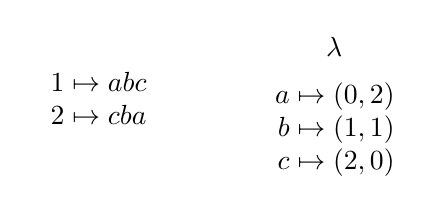
\begin{tikzpicture}
			\path node (P) {$\prof$};
			\path (P.south) node[anchor=north] (profile) {$%
				\begin{array}{r@{\hspace{1mm} \mapsto \hspace{1mm}}l}
					1 & a \pref b \pref c\\%
					2 & c \pref b \pref a\\%
				\end{array}%
			$};
			\path (P.center) ++ (3cm, 0) node (L) {$\lambda_{\prof}$};
			\path (L.south) node[anchor=north] (losses) {$%
				\begin{array}{r@{\hspace{1mm} \mapsto \hspace{1mm}}l}
					a & (0, 2)\\%
					b & (1, 1)\\%
					c & (2, 0)\\%
				\end{array}%
			$};
		\end{tikzpicture}
	\end{example}

	Given $\prof = (\prefi)_{i \in N}$:
	\begin{itemize}
		\item $\lambda_{\prefi}(x) = \card{\set{y \in \allalts \suchthat y \prefi x}} \in \intvl{0, m - 1}$ the loss endured by $i$ when choosing $x \in \allalts$ instead of her favorite alternative
		\item $\lambda_{\prof}: \allalts → \intvl{0, m - 1}^\voters$ s.t. $\lambda_{\prof}(x)$ associates to each voter her loss when choosing $x$
	\end{itemize}
\end{frame}

\begin{frame}
	\frametitle{Inequality}
	\begin{itemize}
		\item We require an inequality measure $\sigma$
		\item Orders completely the loss vectors in $\intvl{0, m - 1}^N$
		\item In order to pick the least unequal loss vectors in $\lambda_{\prof}$
	\end{itemize}
	\begin{block}{Inequality measure}
		\begin{itemize}
			\item $\sigma: \intvl{0, m - 1}^N → \R^+$
			\item $\sigma(l) = 0 ⇔ l = (k)_{i \in N}$ for some $k \in \intvl{0, m - 1}$
			\item $\Sigma$ the set of $\sigma$ satisfying the above
		\end{itemize}
	\end{block}
\end{frame}

\begin{frame}[fragile]
	\frametitle{Minimizing loss vectors}
	Given $\alts \subseteq \allalts$ and $g: \alts → \R$,
	\begin{align}
		\argmin_{x \in \alts}g(x) &= \set{x \in \alts \suchthat g(x) ≤ g(y), \forall y \in \alts}\\
		&= \argmin_\alts g
	\end{align}
	\begin{example}[A profile, its loss vectors and the $\sigma$-minimizer]
		\centering
		\begin{tikzpicture}
			\path node (P) {$\prof$};
			\path (P.south) node[anchor=north] (profile) {$%
				\begin{array}{r@{\hspace{1mm} \mapsto \hspace{1mm}}l}
					1 & a \pref b \pref c\\%
					2 & c \pref b \pref a\\%
				\end{array}%
			$};
			\path (P.center) ++ (3cm, 0) node (L) {$\lambda_{\prof}$};
			\path (L.south) node[anchor=north] (losses) {$%
				\begin{array}{r@{\hspace{1mm} \mapsto \hspace{1mm}}l}
					a & (0, 2)\\%
					b & (1, 1)\\%
					c & (2, 0)\\%
				\end{array}%
			$};
			\path[draw, ->] (P) to (L);
			\path (losses.south) ++ (0, -1cm) coordinate (h2);
			\path ($(P)!.5!(L)$) coordinate (v2);
			\path (h2 -| v2) node (S) {{\visible<1>{\makebox[0pt]{\hspace{3ex}?}}}{\visible<2->{$\set{b}$}}};
			\path[draw, ->] (losses.south) -- (S) node[pos=0.5, anchor=north west, inner sep=0, outer sep=0] {$\argmin_{x \in \allalts} \sigma(\lambda_{\prof}(x))$};
			\onslide<3>{
				\path[draw, ->] (profile.south) -- (S) node[pos=0.5, anchor=north east, inner sep=0, outer sep=0] {$\argmin_{\allalts} (\sigma \circ \lambda_{\prof})$};
			}
		\end{tikzpicture}
	\end{example}
\end{frame}

\subsection{Egalitarian compromises}
\begin{frame}
	\frametitle{Egalitarian compromises}
	An \ac{SCR} is \ac{ECC} iff at each profile, it selects some “minimally inegalitarian” alternative.
	\begin{block}{Egalitarian compromise compatibility}
		An \ac{SCR} $f$ is \ac{ECC} iff 
		\begin{equation}
			\exists \sigma \in \Sigma \suchthat \forall \prof \in \linors^N: f(\prof) \cap \argmin_\allalts (\sigma \circ \lambda_{\prof}) ≠ \emptyset
		\end{equation}
	\end{block}
\end{frame}

\begin{frame}[fragile]
	\frametitle{Paretianism}
	\begin{block}{Paretian rules}
		\begin{itemize}
			\item $\PD(\prof) = \set{x \in \allalts \suchthat \exists y \in \allalts \suchthat y \prefi x, \forall i \in N}$
			\item $\PO(\prof) = \allalts \setminus \PD(\prof)$
			\item An \ac{SCR} $f$ is Paretian iff $\forall \prof \in \linors^N: f(\prof) \subseteq \PO(\prof)$
		\end{itemize}
	\end{block}
	\begin{example}
		$\begin{array}{r@{\hspace{1mm} \mapsto \hspace{1mm}}l}
			1 & a \pref c \pref b \pref d\\%
			2 & c \pref d \pref a \pref b\\%
		\end{array}$%
		\hspace{2cm} $\PD = \only<1>{\text{?}}\onslide<2>{\set{b, d}}$
	\end{example}
\end{frame}

\begin{frame}[fragile]
	\frametitle{Equality and Pareto dominance}
	\ac{ECC} rules are \emph{very} egalitarian
	\begin{example}
		\centering
		\begin{tikzpicture}
			\path node (P) {$\prof$};
			\path (P.south) node[anchor=north] (profile) {$%
				\begin{array}{r@{\hspace{1mm} \mapsto \hspace{1mm}}l}
					1 & a \pref c \pref b\\%
					2 & c \pref a \pref b\\%
				\end{array}%
			$};
			\onslide<2>{
				\path (P.center) ++ (3cm, 0) node (L) {$\lambda_{\prof}$};
				\path (L.south) node[anchor=north] (losses) {$%
					\begin{array}{r@{\hspace{1mm} \mapsto \hspace{1mm}}l}
						a & (0, 1)\\%
						b & (2, 2)\\%
						c & (1, 0)\\%
					\end{array}%
				$};
				\path[draw, ->] (P) to (L);
				\path (losses.south) ++ (0, -1cm) coordinate (h2);
				\path ($(P)!.5!(L)$) coordinate (v2);
				\path (h2 -| v2) node (S) {$\set{b}$};
				\path[draw, ->] (losses.south) -- (S) node[pos=0.5, anchor=north west, inner sep=0, outer sep=0] {$\argmin_{x \in \allalts} \sigma(\lambda_{\prof}(x))$};
				\path[draw, ->] (profile.south) -- (S) node[pos=0.5, anchor=north east, inner sep=0, outer sep=0] {$\argmin_{\allalts} (\sigma \circ \lambda_{\prof})$};
			}
		\end{tikzpicture}
	\end{example}
	\onslide<2>{Egalitarian compromises favor equality over Pareto efficiency}
\end{frame}

\begin{frame}
	\frametitle{ECC $\cap$ Paretian = $\emptyset$}
	I write ECC for the set of \acp{SCR} satisfying ECC, and similarly for other properties
	\begin{theorem}
		ECC $\cap$ Paretian = $\emptyset$ \hfill {\small (for $n, m ≥ 2$)}
	\end{theorem}
	\begin{proof}[Proof (for $m$ = 4; adaptations for any $m ≥ 2$ are straightforward)]
		$\begin{array}{r@{}l@{\hspace{1mm} \mapsto \hspace{1mm}}l}
			1 &\text{ voter} & a_1 \pref a_2 \pref a_3 \pref x\\%
			n - 1 &\text{ voters} & a_2 \pref a_3 \pref a_1 \pref x\\%
		\end{array}$%
		\begin{itemize}
			\item $\forall \sigma \in \Sigma: \argmin_\allalts (\sigma \circ \lambda_{\prof}) = \set{x}$
			\item $f \in \text{ECC} ⇒ x \in f(\prof)$
			\item $f \in \text{Paretian} ⇒ x \notin f(\prof)$ \qedhere
		\end{itemize}
	\end{proof}
\end{frame}

\subsection{Paretian compromises}
\begin{frame}
	\frametitle{Paretian compromises}
	An \ac{SCR} is \ac{PCC} iff at each profile, it selects some “minimally inegalitarian” alternative \emph{among the Pareto optimal ones}.
	\begin{block}{Paretian optimal compatibility}
		An \ac{SCR} $f$ is \ac{PCC} iff 
		\begin{equation}
			\exists \sigma \in \Sigma \suchthat \forall \prof \in \linors^N: f(\prof) \cap \argmin_{\PO(\prof)} (\sigma \circ \lambda_{\prof}) ≠ \emptyset
		\end{equation}
	\end{block}
	Recall:
	\begin{block}{Egalitarian compromise compatibility}
		An \ac{SCR} $f$ is \ac{ECC} iff 
		\begin{equation}
			\exists \sigma \in \Sigma \suchthat \forall \prof \in \linors^N: f(\prof) \cap \argmin_\allalts (\sigma \circ \lambda_{\prof}) ≠ \emptyset
		\end{equation}
	\end{block}
\end{frame}

\subsection{Two remarks}
\begin{frame}
	\frametitle{Paretian compromises and Paretianism}
	PCC does not \emph{require} Paretianism, but is \emph{compatible} with it.
	\begin{itemize}
		\item PCC $\not⇒$ Paretian
		\begin{itemize}
			\item Consider $f(\prof) = \allalts$
			\item $f$ is PCC and $f$ is not Paretian
		\end{itemize}
		\item PCC does not require to select \emph{only} among $\PO(\prof)$
		\item PCC requires to select \emph{some} {(most equal)} alt.\ among $\PO(\prof)$
	\end{itemize}
\end{frame}

%\begin{frame}
%	\frametitle{PCC rules are still very pro-egalitarian}
%	\begin{example}[PCC]
%		$\begin{array}{rl}
%			n - 1 \text{ voters} & a \pref b \pref c\\%
%			1 \text{ voter} & c \pref b \pref a\\%
%		\end{array}$
%		\hspace{2cm} PCC selects? \onslide<2>{$\set{b}$
%	\end{example}
%\end{frame}

\begin{frame}[fragile]
	\frametitle{About our inequality measures}
	Note that $\Sigma$ contains \emph{all} inequality measures that say that constant vectors are the most equal of all.
	\begin{example}[Constraint imposed by PCC]
		\begin{center}
			\begin{tikzpicture}
				\path node (P) {$\prof$};
				\path (P.south) node[anchor=north] (profile) {$%
					\begin{array}{r@{\hspace{1mm} \mapsto \hspace{1mm}}l}
						1 & a \pref b \pref c \pref d\\%
						2 & d \pref a \pref c \pref b\\%
					\end{array}%
				$};
				\onslide<2>{
					\path (P.center) ++ (4cm, 0) node (L) {$\lambda_{\prof}$};
					\path (L.south) node[anchor=north] (losses) {$%
						\begin{array}{r@{\hspace{1mm} \mapsto \hspace{1mm}}l}
							a & (0, 1)\\%
							d & (3, 0)\\%
						\end{array}%
					$};
					\path (losses.south) ++ (0, -1cm) coordinate (h2);
					\path ($(P)!.5!(L)$) coordinate (v2);
					\path (h2 -| v2) node (S) {$\subseteq \set{a, d}$};
					\path[draw, ->] (losses.south) -- (S) node[pos=0.5, anchor=north west, inner sep=0, outer sep=0] {$\argmin_{x \in \PO(\prof)} \sigma(\lambda_{\prof}(x))$};
					\path[draw, ->] (profile.south) -- (S) node[pos=0.5, anchor=north east, inner sep=0, outer sep=0] {$\argmin_{\PO(\prof)} (\sigma \circ \lambda_{\prof})$};
				}
			\end{tikzpicture}
		\end{center}
		\onslide<2>{A PCC $f$ must pick at least one among $a$ and $d$ (depending on $\sigma$)}
	\end{example}
\end{frame}

\section{Comparison}
\subsection{BK compromises}
\begin{frame}
	\frametitle{BK compromise}
	\citet{Brams2001} compromise
	\begin{itemize}
		\item Denoted by $\BK[q]$, with $q \in \intvl{1, n}$
		\item A voter \emph{supports} an alternative at rank $r$ iff she places this alternative at $r$ or better
		\item $\rho_q$: best rank for which some alternative receives $≥ q$ supports
		\item $\BK$ selects the best supported alternatives at rank $\rho_q$
	\end{itemize}
	\begin{example}[{$\BK[3]$}]
		$\begin{array}{r@{\hspace{1mm} \mapsto \hspace{1mm}}l}
			1 & a \pref b \pref c \pref d\\%
			2 & c \pref b \pref a \pref d\\%
			3 & b \pref c \pref d \pref a\\%
			4 & c \pref a \pref d \pref b\\%
			5 & d \pref c \pref b \pref a\\%
		\end{array}$
		\hspace{2cm} $\BK[3]$ selects? \onslide<2>{$\set{c}$ ($\rho_3 = 2$)}
	\end{example}
\end{frame}

\begin{frame}
	\frametitle{Sorts of BK compromises}
	$\BK[\ceil{n / 2}]$ : Majoritarian compromise \citep{Sertel1999} (also “Bucklin” \citep{Erdelyi2015})
	\begin{block}{\citet[abstract]{Sertel1999}}
		\og{}The Majoritarian Compromise is “majoritarian approving” i.e. it always picks “what’s good for a majority” (alternatives which some majority regards as among the better “effective” half of the available alternatives).\fg{}
	\end{block}
	$\BK[n]$: Fallback bargaining
%	\begin{itemize}
%		\item $\rho_n$: the best rank at which some alternative receives unanimous support. $\BK[n]$ selects the best supported alternatives at rank $\rho_n$.
%	\end{itemize}
	\begin{example}[${\BK[n]}$]
		$\begin{array}{rl}
			3 \text{ voters} & a_1 \pref a_2 \pref a_3 \pref a_4\\%
			2 \text{ voters} & a_2 \pref a_1 \pref a_4 \pref a_3\\%
		\end{array}$
		\hspace{2cm} $\BK[n]$ selects? \onslide<2>{$\set{a_1, a_2}$}
	\end{example}
\end{frame}

\begin{frame}
	\frametitle{$\BK, q \in \intvl{1, n}$ is not ECC}
	\begin{theorem}
		$\BK$ is not ECC.\hfill {\small (for $m, n ≥ 2$)}
	\end{theorem}
	\begin{proof}
		$\BK$ is Paretian: consider an alternative $x$ supported by voters $V \subseteq N$ at some rank $r$ and $y \prefi x, \forall i \in V$. Then, the voters in $V$ support $y$ at rank $r$, and never rank $y$ at rank $r$ (as $x$ is at rank $r$ or better). Thus, $V$ supported $y$ already at a better rank. 
		
		The winners in $\BK$ gather $q' ≥ q$ supports at $\rho_q$, and any Pareto-dominating alternative would gather $q' ≥ q$ supports at a better rank. Thus, $\BK$ may not select a Pareto-dominated alternative.
	\end{proof}
\end{frame}

\begin{frame}
	\frametitle{BK compromises (q ≠ n) are not PCC}
	\begin{theorem}
		$\BK, q \in \intvl{1, n - 1}$ is neither ECC nor PCC.\hfill {\small (for $m ≥ 3, n ≥ 2$)}
	\end{theorem}
	\begin{proof}
		$\begin{array}{r@{}l@{\hspace{1mm} \mapsto \hspace{1mm}}l}
			n - 1 &\text{ voters} & x \pref y \pref z \pref …\\%
			1 &\text{ voter} & z \pref y \pref … \pref x\\%
		\end{array}$%
		\begin{itemize}
			\item $\rho_q = 1$ thus $y \notin \BK(\prof)$
			\item $\argmin_{\allalts} (\sigma \circ \lprof) = \set{y}$, thus $f \in ECC ⇒ y \in f(\prof)$
			\item $\argmin_{\PO(\prof)} (\sigma \circ \lprof) = \set{y}$, thus $f \in PCC ⇒ y \in f(\prof)$\qedhere
		\end{itemize}
	\end{proof}
	(This also proves more directly that $\BK, q \in \intvl{1, n - 1}$ fails ECC)
\end{frame}

\begin{frame}
	\frametitle{$\BK[n]$ is PCC}
	Showing that $\BK[n]$ is not PCC requires to restrict $\Sigma$
	\begin{theorem}
		$\BK[n]$ is PCC.
	\end{theorem}
	\begin{proof}[Proof sketch]
		Define $\sigma^\text{discrete}(l) = 1 ⇔ l$ is not constant.
		We prove that $\BK[n] \subseteq \argmin_{\PO(\prof)} (\sigma^\text{discrete} \circ \lprof)$.
		
		If some $x \in \PO(\prof)$ has a constant loss vector, e.\ g.\ $\begin{array}{l}
			a_1 \pref a_2 \pref a_3 \pref a_4 \pref a_5 \pref a_6\\
			a_5 \pref a_4 \pref a_3 \pref a_1 \pref a_2 \pref a_6\\
		\end{array}$, there is exactly one such alternative, $\rho_n$ is its rank, and $\BK[n](\prof) = \set{x}$.

		Otherwise, $\sigma$ does not discriminate among $\PO(\prof)$, thus Paretianism suffices.
	\end{proof}
\end{frame}

\subsection{Condorcet rules}
\begin{frame}
	\frametitle{Condorcet rules}
	$f$ is Condorcet consistent iff $[x \text{ is the Condorcet winner in } \prof ⇒ f(\prof) = \set{x}]$
	\begin{theorem}
		A Condorcet consistent $f$ is neither ECC nor PCC.\hfill {\small (for $m, n ≥ 3$)}
	\end{theorem}
	\begin{proof}
		$\begin{array}{r@{}l@{\hspace{1mm} \mapsto \hspace{1mm}}l}
			n - 1 &\text{ voters} & x \pref y \pref z \pref …\\%
			1 &\text{ voter} & z \pref y \pref … \pref x\\%
		\end{array}$%
		\begin{itemize}
			\item $f$ Condorcet consistent $⇒ f(\prof) = \set{x}$
			\item $f$ ECC $⇒ y \in f(\prof)$
			\item $f$ PCC $⇒ y \in f(\prof)$\qedhere
		\end{itemize}
	\end{proof}
\end{frame}

\subsection{Scoring rules}
\begin{frame}
	\frametitle{Scoring rule}
	\begin{example}[Scoring]
		Given $w = (3, 2, 0)$
		\begin{center}
			\vspace{-3mm}
			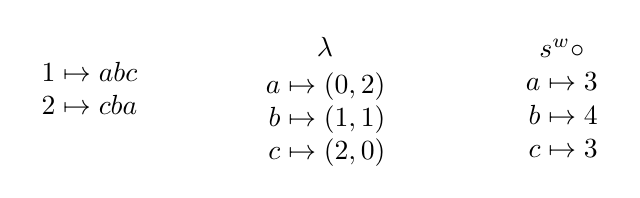
\begin{tikzpicture}
				\path node (P) {$\prof$};
				\path (P.south) node[anchor=north, inner sep=0, outer sep=0] (profile) {$%
					\begin{array}{r@{\hspace{1mm} \mapsto \hspace{1mm}}l}
						1 & a \pref b \pref c\\%
						2 & c \pref b \pref a\\%
					\end{array}%
				$};
				\path (P.center) ++ (3cm, 0) node (L) {$\lambda_{\prof}$};
				\path (L.south) node[anchor=north, inner sep=0, outer sep=0] (losses) {$%
					\begin{array}{r@{\hspace{1mm} \mapsto \hspace{1mm}}l}
						a & (0, 2)\\%
						b & (1, 1)\\%
						c & (2, 0)\\%
					\end{array}%
				$};
				\path (L) ++ (3cm, 0) node (s) {$s^w \circ \lprof$};
				\path (s.south) node[anchor=north, inner sep=0, outer sep=0] (scores) {$%
					\begin{array}{r@{\hspace{1mm} \mapsto \hspace{1mm}}l}
						a & 3\\%
						b & 4\\%
						c & 3\\%
					\end{array}%
				$};
			\end{tikzpicture}
		\end{center}
	\end{example}
	\begin{itemize}
		\item A \emph{weight vector} $w \in \R^{\intvl{0, m - 1}}$ associates a weight to every possible loss
		\item With higher weights for lower losses: $\forall j \in \intvl{0, m - 2}$, $w_j ≥ w_{j + 1}$, and $w_0 ≠ w_{m - 1}$
		\item Score associated to loss vector $(l_k)_{k \in N}$ is $s^w(l) = \sum_{k \in N} w_{l_k}$
		\item $w$ determines the scoring rule $f^w = \argmax_\allalts (s^w \circ \lambda_{\prof})$ that picks those alternatives having highest-scoring loss vectors.
	\end{itemize}
\end{frame}

\begin{frame}
	\frametitle{Scoring rules are not ECC}
	\begin{theorem}
		Consider any weight vector $w$ with $w_j ≥ w_{j + 1}$, and $w_0 ≠ w_{m - 1}$. $f^w$ is not ECC.
		\hfill {\small (for $m, n ≥ 2$)}
	\end{theorem}
	\begin{proof}[Proof (for $m$ = 4; adaptations for any $m ≥ 2$ are straightforward)]
		$\begin{array}{r@{}l@{\hspace{1mm} \mapsto \hspace{1mm}}l}
			1 &\text{ voter} & a_1 \pref a_2 \pref a_3 \pref x\\%
			n - 1 &\text{ voters} & a_2 \pref a_3 \pref a_1 \pref x\\%
		\end{array}$%
		\begin{itemize}
			\item $\argmin_\allalts (\sigma \circ \lambda_{\prof}) = \set{x}$, thus $f \in ECC ⇒ x \in f(\prof)$
			\item $(s \circ \lprof)(x) < (s \circ \lprof)(a_1)$, thus $x \notin f^w(\prof)$ \qedhere
		\end{itemize}
	\end{proof}
\end{frame}

\begin{frame}
	\frametitle{Anti-plurality}
	\begin{itemize}
		\item $w$ is an Anti-plurality (AP) weight vector iff $w_0 = w_{m - 2}$.
		\item Example: $w = (3, 3, 3, 0)$
	\end{itemize}
	\begin{theorem}
		Given an AP $w$, $f^w$ is PCC \hfill {\small (for $m ≥ 2$)}
	\end{theorem}
	\begin{proof}[Proof idea]
		Define $\sigma^\text{discrete}(l) = 1 ⇔ l$ is not constant.
		To prove: $\exists x \in f^w(\prof) \cap \argmin_{\PO(\prof)} (\sigma^\text{discrete} \circ \lprof)$.
		
		Assume $\prof$ contains some $x \in \PO(\prof)$ with a constant loss vector, e.\ g.\ 
		$\begin{array}{l}
			a_1 \pref a_2 \pref a_3 \pref a_4\\
			a_3 \pref a_2 \pref a_1 \pref a_4\\
		\end{array}$.
		This $x$ is never last, so $x \in f^w(\prof)$.
		
		Otherwise, $\sigma$ does not discriminate among $\PO(\prof)$. Take any $x \in \PO(\prof) \cap f^w$.
	\end{proof}
\end{frame}

\begin{frame}
	\frametitle{Scoring rules not AP are not PCC for large enough $n$}
	\begin{theorem}
		Given a non AP $w$, $m ≥ 3$ and a large enough $n$, $f^w$ is not PCC.
	\end{theorem}
	\begin{proof}[Sketch of proof]
		$\begin{array}{rl}
			i = 1 & a_2 \pref … \pref a_m \pref a_1\\%
			2 ≤ i ≤ m - 2 & a_1 \pref … \pref a_m \pref a_i\\%
			m - 1 ≤ i ≤ n & a_1 \pref … \pref a_m \pref a_{m - 1}\\%
		\end{array}$%
		\begin{itemize}
			\item $\argmin_{\PO(\prof)} (\sigma \circ \lprof) = \set{a_m}$, thus $f \in PCC ⇒ a_m \in f(\prof)$
			\item For $n$ large enough, $(s \circ \lprof)(a_1) > (s \circ \lprof)(a_m)$, thus $a_m \notin f^w(\prof)$ \qedhere
		\end{itemize}
	\end{proof}
	We see that PCC rules are \emph{very} egalitarian
\end{frame}

\subsection{Restricting \texorpdfstring{$\Sigma$}{Sigma}}
\begin{frame}
	\frametitle{Restricting $\Sigma$}
	\begin{itemize}
		\item Among the rules seen here, only $\BK[n]$ and Anti-plurality are PCC
		\item Proved using a “weird” $\sigma$ inequality measure
		\item This positive result vanishes with a slight supplementary restriction on $\Sigma$
	\end{itemize}
	\begin{definition}[Condition $C_{m, n}$]
		Given $m ≥ 4, n ≥ \max\set{4, m - 1}$, $\sigma$ satisfies condition $C_{m, n}$ iff $\sigma(m - 3, m - 1, m - 2, …, m - 2) < \sigma(m - 2, m - 3, …, 1, 0, …, 0)$.
	\end{definition}
	\begin{example}%[Examples of conditions $C$]
		$C_{5, 4}$ requires $\sigma(2, 4, 3, 3) < \sigma(3, 2, 1, 0)$.

		$C_{6, 5}$ requires $\sigma(3, 5, 4, 4, 4) < \sigma(4, 3, 2, 1, 0)$.
	\end{example}
\end{frame}

\begin{frame}
	\frametitle{Under condition \texorpdfstring{$C_{m, n}$}{C(m, n)}}
	\begin{theorem}
		Under condition $C_{m, n}$, and  given an AP $w$, $\BK[n]$ and $f^w$ $\notin$ PCC.
	\end{theorem}
	\begin{proof}[Proof for $m = 5, n = 4$]
		$\begin{array}{r@{\hspace{1mm} \mapsto \hspace{1mm}}lllll}
			1 &	&	&x	&y	&a_1\\%
			2 &	&	&y	&	&x\\%
			3 &	&y	&	&x	&a_2\\%
			4 &y	&	&	&x	&a_3\\%
		\end{array}$%
		\begin{itemize}
			\item $y$ is the only alt.\ never last, thus for both rules: $f(\prof) = \set{y}$
			\item $\lprof(x) = (2, 4, 3, 3)$, $\lprof(y) = (3, 2, 1, 0)$ thus $(\sigma \circ \lprof)(x) < (\sigma \circ \lprof)(y)$
			\item and $x \in \PO(\prof)$, thus $y \notin \argmin_{\PO(\prof)}(\sigma \circ \lprof)$ \qedhere
		\end{itemize}
	\end{proof}
	We see (again) that PCC rules are \emph{very} egalitarian
\end{frame}

\section{Two individuals}
\subsection{\texorpdfstring{$\BK[n = 2]$}{BK for two individuals}}
\begin{frame}
	\frametitle{Bargaining contexts}
	\begin{itemize}
		\item We see that our compromise rules place an important emphasis on equality
		\item This might be particularly justified in bargaining contexts
		\item Appears comparatively harder to justify in voting contexts
		\item \citet{Brams2001} indicate that they recommend the rule $\BK[n]$ particularly in bargaining contexts
		\item Let’s see how $\BK[n = 2]$ relate to PCC
	\end{itemize}
\end{frame}

\begin{frame}
	\frametitle{Restricting $\Sigma$ for two individuals}
	Showing that $\BK[n = 2]$ is not PCC requires to restrict $\Sigma$
	\begin{definition}[Condition $D_m$]
		Given $m ≥ 7$ odd, $\sigma$ satisfies condition $D_m$ iff $\sigma(\frac{m - 1}{2} + 1, \frac{m - 1}{2} - 1) < \sigma(0, \frac{m - 1}{2})$
	\end{definition}
	\begin{example}
		$D_7$ requires $\sigma(4, 2) < \sigma(0, 3)$

		$D_9$ requires $\sigma(5, 3) < \sigma(0, 4)$
	\end{example}
\end{frame}

\begin{frame}
	\frametitle{$\BK[n = 2]$ is not PCC under condition $D$}
	\label{sl:bknnotpcc}
	\begin{theorem}
		Given $m ≥ 7$ odd and $n = 2$, under condition $D_m$, $\BK[n]$ is not PCC.
	\end{theorem}
	\begin{proof}[Proof \hfill {\small [illustrations for $m = 9$]}]
		Define $\alpha = \frac{m - 1}{2}$, $\beta = \frac{m - 1}{2} - 1$ \hfill {\small [$\alpha = 4, \beta = 3$]}

		$\begin{array}{r@{\hspace{1mm} \mapsto \hspace{1mm}}lllllllll}
			1 & x &\pref a_1 &\pref a_2 &\pref … &\pref a_\alpha &\pref y &\pref b_1 &\pref … &\pref b_\beta\\
			2 & b_1 &\pref … &\pref b_\beta &\pref y &\pref x &\pref a_1 &\pref a_2 &\pref … &\pref a_\alpha\\
		\end{array}$%
		\begin{itemize} 
			\item $\BK[n] = \set{x}$
			\item $\lprof(y) = (\alpha + 1, \beta)$, $\lprof(x) = (0, \beta + 1)$ thus $(\sigma \circ \lprof)(y) < (\sigma \circ \lprof)(x)$ \hfill {\small [$\lprof(y) = (5, 3)$, $\lprof(x) = (0, 4)$]}
			\item and $y \in \PO(\prof)$, thus $x \notin \argmin_{\PO(\prof)}(\sigma \circ \lprof)$ \qedhere
		\end{itemize}
	\end{proof}
\end{frame}

\subsection{Other rules}
\begin{frame}
	\frametitle{Other two person bargaining rules}
	Similar results hold for: 
	\begin{itemize}
		\item $\BK[n]$, $m$ even
		\item Pareto-and-Veto rules \citep{Laslier2020}
		\item Veto-Rank mechanism \citep{Clippel2014}
		\item Shortlisting \citep{Clippel2014}
	\end{itemize}
	The proofs are very similar to the one just shown.
\end{frame}

\subsection{Discussion}
\begin{frame}
	\frametitle{Discussion}
	\begin{itemize}
		\item Our compromises try to make everybody concede equally
		\item Disagree with many rules
		\item Might be considered too egalitarian, but (I’d argue) interesting to study conceptually
		\item Might lead to question Pareto in favor of equality (already studied?)
		\item Possibly fitting some bargaining behavior (think about ultimatum games)
	\end{itemize}
\end{frame}

\begin{frame}[plain]
	\addtocounter{framenumber}{-1}
	\begin{center}
		\huge
		\textit{Thank you for your attention!}
	\end{center}
\end{frame}

\appendix
\AtBeginSection{
}
%- Appendix: I put a before b from my own perspective; but considering 1’s POV, I prefer b to a: either because I am envious, or even one could say that my objective interest is that b > a, even when I ignore that a is there. When my pref chg because of someone else, it is considered envy, but it may be about my interest.
%- Not ashamed of this very egalitarian focus but we’re willing to compromise to cope with classical demands of our fellow economist colleagues.

\section{Plurality}
\begin{frame}
	\frametitle{Plurality}
	Plurality selects the alternatives most often at first rank
	\begin{example}[Plurality]
		$\begin{array}{r@{\hspace{1mm} \mapsto \hspace{1mm}}l}
			1 & a \pref b \pref c \pref d\\%
			2 & a \pref b \pref c \pref d\\%
			3 & b \pref c \pref d \pref a\\%
			4 & c \pref b \pref d \pref a\\%
			5 & d \pref b \pref c \pref a\\%
		\end{array}$
		\hspace{2cm} Plurality selects? \onslide<2>{$\set{a}$}
		
		\vspace{1em}
		Here, Plurality only “considers” a minority of individuals.
	\end{example}
\end{frame}

\section{Ex-ante compromises}
\begin{frame}
	\frametitle{A compromise may be exclusively ex-ante}
	\begin{example}[{$\BK[51]$}]
		$\begin{array}{rl}
			49\text{ voters} & a \pref b \pref c\\%
			51\text{ voters} & c \pref b \pref a\\%
		\end{array}$
		\hspace{2cm} $\BK[51]$ selects? \onslide<2>{$\set{c}$ ($\rho_{51} = 1$)}
	\end{example}
	\begin{itemize}
		\item Actually \emph{nobody} conceded anything here
		\item “Ex-ante” compromise: a priori willingness to compromise may not require compromising
		\item Observation holds for any $q \in \intvl{1, n - 1}$
		\item See Slide \ref{sl:bknnotpcc} for an application to the case $q = n$
	\end{itemize}
\end{frame}

%\clearpage\pdfbookmark[2]{\refname}{\refname}
\begin{frame}[allowframebreaks]
	\frametitle{\refname}
 	\bibliography{biblio}
\end{frame}

\clearpage\pdfbookmark[2]{License}{License}
\begin{frame}[plain]
	\frametitle{License}
	This presentation, and the associated \LaTeX{} code, are published under the \href{https://opensource.org/licenses/MIT}{MIT license}. Feel free to reuse (parts of) the presentation, under condition that you cite the author.
	
	Credits are to be given to \hrefblue{https://www.lamsade.dauphine.fr/~ocailloux/}{Olivier Cailloux}, Université Paris-Dauphine.
\end{frame}
\addtocounter{framenumber}{-1}
\end{document}

\begin{frame}
	\frametitle{Title}
	\begin{block}{Block}
%		\setlength\abovedisplayskip{1 ex}% reduce space above equations
		\begin{itemize}
			\item Item
		\end{itemize}
	\end{block}
	\begin{itemize}
		\item Item
	\end{itemize}
\end{frame}

